\chapter{COMMISSIONING ST.\ GEORGE}

The St.\ George recoil mass separator was designed to have an energy acceptance
of $\Delta E/E = \pm7.5$\,\% and an angular acceptance of
$\Delta\theta = \pm40$~mrad, based on the kinematics of a set of
astrophysically important $(\alpha,\gamma)$ reactions~(\cite{Couder2008} and
Section~\ref{sec:stg}).
% The total acceptance, i.e.\ the combined angular and energy acceptance, must be
% determined experimentally through direct beam studies, simulating reaction
% products with a degrading foil, or actually performing a reaction study.
The ion optics that maximize the acceptance of the recoil particles and the
rejection and suppression of the beam particles must be experimentally
determined. The calculated ion optics are related to those achieved
experimentally through the measured performance of the recoil separator. By
measuring the acceptance achieved through various tunes and techniques is one
way to determine if the desired calculated transport properties have or have
not been achieved experimentally.
Recently, the energy acceptance was initially studied separately from the
angular acceptance (published in \cite{Meisel2017}) to provide a relation
between the predicted and experimentally determined field values. The angular
acceptance was studied through a variety of methods, both in conjunction and
without a corresponding energy acceptance requirement. Measuring the acceptance
of a separator is paramount to using it for experimental measurements.

Two primary commissioning campaigns, determining the angular and energy
acceptances for a given desired global setting of the separator, have been
undertaken. The two global settings are: (i) the designed parameters for St.\
George for transporting heavy recoil products produced by $(\alpha,\gamma)$
reactions in inverse kinematics through the entire separator, and (ii) the
altered parameters for transporting $\alpha$ particles produced by
$(\textrm{p},\alpha)$ reactions in forward kinematics to focal plane $F_2$.
From each global setting, the separator elements can be scaled based on the
desired transport particle's magnetic (Eq.~\ref{eq:brho}) and electric
(Eq.~\ref{eq:erho}) rigidities. The experimentally determined values after
scaling from the global setting may differ from the predicted scaled values
when scaled over a large range, requiring multiple rigidities within the
allowed rigidity phase space to be explored to fully commission the separator.
For the
altered forward kinematics separator settings, due to the relatively small
rigidity phase space the initial test reaction covers and the fact that a
direct $\alpha$ beam can be used, the element field strengths were directly
determined prior to the data collection experiment.

For the designed inverse kinematics separator settings, various beams spanning
a large region within the desired rigidity phase space were used. Test beams
included light beams (\nuc{1}{H} and \nuc{4}{He}) due to their ease of
production and heavier beams (\nuc{16}{O} and \nuc{20}{Ne}) to simulate
transporting heavy reaction products through the separator. Beam particle,
charge state, and energy were limited by the capabilities of the 5U to produce
the desired beam. The commissioning
work was divided between focusing on the energy or angular acceptance
relatively independent of the other. For some of the angular acceptance
measurements, a small energy spread was included to better recreate the
conditions under which St.\ George will be used.


\begin{figure}
    \begin{center}
        \centerline{
            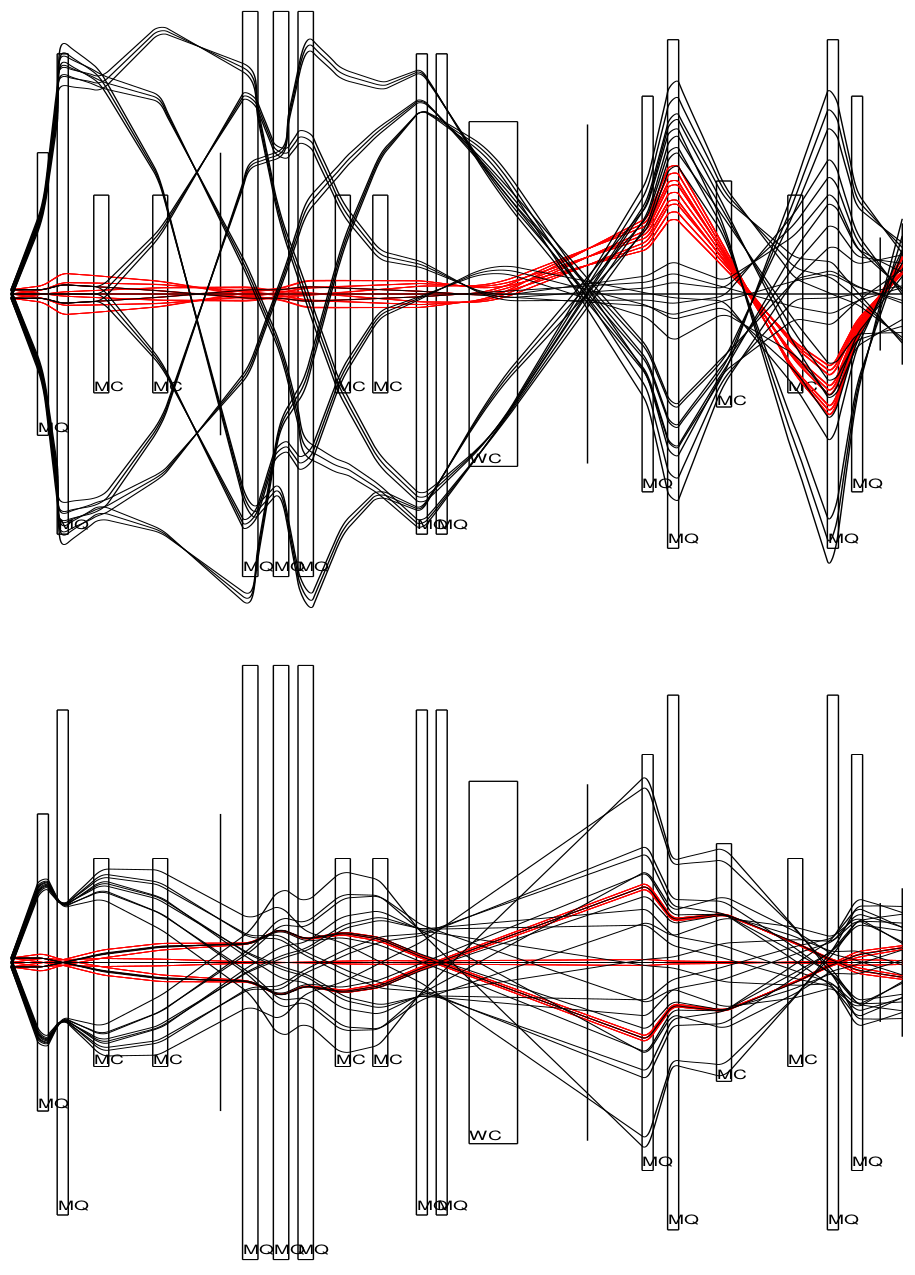
\includegraphics[width=0.8\textwidth]{figures/raytrace.png}}
        \caption[Horizontal and vertical rays through St.\ George]{Horizontal
            (upper plot) and vertical (lower plot) rays through St.\ George.
            Recoil \nuc{41}{Sc} rays are shown in black and beam \nuc{40}{Ca}
            rays are shown in red.
            % The beam energy is
            % $E_{\textrm{beam}} = 15.99\pm0.001$~MeV, and the recoil energy is
            % $E_{\textrm{recoil}} = 15.6\pm1.155$~MeV.
            The beam rigidities are $B\rho = 0.331$~Tm and $E\rho = 2.907$~MV,
            and the recoil rigidities are $B\rho = 0.331$~Tm and
            $E\rho = 2.836$~MV. Both the beam and recoil
            are taken to be in the $11^+$ charge state.
            The COSY calculation assumes that the recoil particles are spread
            within an acceptance range of $\Delta E/E \approx7.5$\,\% and
            $\Delta\theta = 40$~mrad. The transverse scale is highly
            exaggerated to show detail.}
        \label{fig:raytrace}
    \end{center}
\end{figure}


\section{Theoretical and Experimental Considerations}
\label{sec:cosy}

% Possibly move this to Chapter 2...

St.\ George was modeled within COSY Infinity (COSY-$\infty$, henceforth
\emph{COSY}), a beam optics and transport language developed at Michigan State
University~\cite{COSY}. The initial ion optics solution for the separator was
calculated by
Drs.\ Couder and Berg at the University of Notre Dame to maximize the angular
and energy acceptance for a point-like target located prior to the separator.
Optimization of the individual elements' properties allowed the separator
to achieve the previously-stated energy and angular acceptances, create an
achromatic focus at the mass slits (focal plane $F_2$), and transport all
recoils to the final detector focal plane $F_3$ (see Section~\ref{sec:stg}).
Each magnetic element is represented by a single command within the code,
defining the type and properties of the desired element. The three types of
elements used within St.\ George\----{}dipoles, quadrupoles, and the Wien
filter\----{}require different sets of values to be defined. The recoil
envelope, consisting of a number of sample recoil properties used as
representative rays, for the final designed configuration is shown in
Fig.~\ref{fig:raytrace}. For the example shown, the quadrupole pole tip fields
are given in
Table~\ref{tab:poletip}, where negative values represent a quadrupole focusing
in the $y$-direction. The pole tip fields for $(\alpha,\gamma)$ experiments are
for the test particles shown, while those for $(\rm{p},\gamma)$ experiments are
specific to this work (see Section~[REFERENCE]). The actual fields used will
depend on the rigidity of the desired particle to transport through the
separator and can be scaled from these values.

The initial ion optics solution creates a transport map for particles passing
through the entire separator that can be analyzed independently of the ray
traces and provide the mathematical backing to the particles' trajectories
within St.\ George. The transport map is dependent on the quantities
\begin{equation}
    \label{eq:cosyvars}
    \begin{split}
        r_1 &= x \\
        r_3 &= y \\
        r_5 &= l = -(t - t_0)v_0\gamma/(1 + \gamma) \\
        r_7 &= \delta_m = (m - m_0)/m_0
    \end{split}
    \quad\quad
    \begin{split}
        r_2 &= a = p_x/p_0 \\
        r_4 &= b = p_y/p_0 \\
        r_6 &= \delta_K = (K - K_0)/K_0\\
        r_8 &= \delta_z = (z - z_0)/z_0,
    \end{split}
\end{equation}
where $a$ and $b$ are analogous to angles within each plane, $\delta_K$ is the
energy difference from the desired energy $K_0$,
$\delta_m$ is the mass difference from the desired mass $m_0$, and
$\delta_z$ is the charge from the desired charge state $z_0$~\cite{COSY}.
The desired quantities are the values used to calculate the magnetic
(Eq.~\ref{eq:brho}) and electric (Eq.~\ref{eq:erho}) rigidity, and thus set the
fields of the elements within St.\ George,
of the particle to be transported through the entirety of the separator.
The time of flight difference $l$ is not considered in analyzing the separator.
The transport map contains terms up to fourth order.

The original ion optics calculation used default parameters to describe the
fringe fields of the optical elements. A change in the shape of the fringe
field can change the trajectory of the particles within the separator, as the
total field that the particle interacts with changes in magnitude. Since the
fringe fields used to find the ion optics solution and those created by the
actual magnetic elements within St.\ George may be different, the required
field strength may also be different. The pole tip fields for a given particle
rigidity, determined by the current setpoint for that magnetic, must be found
experimentally, or a new ion optics solution using fringe field
parameterizations that more accurately reflect those exhibited by the magnetic
elements must be found. The procedures for each of the three different types
of elements necessarily differ based on what diagnostic equipment is available.

% This problem really only affects the focusing quadrupoles within the separator.
% While the dipole magnets are set based on the rigidity of the desired particle,
% those magnetic settings can also be determined by observing the trajectory
% within the separator itself. As the overall desire of the dipole magnets is to
% transport the desired rigidity down the center of the separator, diagnostic
% equipment aligned with this central axis can be used to ensure that the beam is
% traveling along this centerline. In doing so, the experimentally correct field
% setting for the dipoles can be determined without too much effort.
The magnetic settings for the dipole magnets, determined by the rigidity of the
particles, can be determined by observing the trajectory of the particles within
the separator, where trajectories close to the central axis are desired. As this
trajectory can be directly observed using diagnostic equipment aligned with the
axis, it is relatively easy for the required values to be found within some
confidence interval around the theoretically desired value. Once these coarse
values are found, the final values which direct the particle beam along the
magnetic optical axis of the following quadrupoles can be determined by
minimizing the off-axis steering effects of the quadrupoles by adjusting the
dipoles' magnetic fields within a small window of values.

Setting the Wien filter can be done in a similar manner. The electric field
strength is determined from the analyzed energy of the particle, the known
charge state, and the desired bending radius of the filter. Thus, the electric
field strength can be set to an exact value, requiring the magnetic field to
be set to match the properties of the electric field. The strength of the
magnetic field is set such that the bending radii of the two fields are the
same and so that the particle beam continues along the magnetic optical axis in
the same manner as described previously with the standard dipoles. The
Wien filter was designed with magnetic yokes at the entrance and exit of the
filter to restrict the magnetic fringe field so that it matches the electric
fringe field created by the electrostatic plates, and those must be adjusted to
their proper positions before the magnetic field can be set.

The magnetic quadrupoles, due to the inability to directly observe the trajectory
of the focused particles within the separator at all possible angles and energies
concurrently to achieve the required acceptance properties of the separator,
require a similarly complicated and restrictive procedure to determine the
experimental settings that match the results of the beam optics calculations.
The full procedure is outlined in \ref{sec:tuning_stg}.


\section{Separator Properties}

The elements, power supplies, and supports were provided by Bruker Biospin and
installed in 200X. The separator design requirements for the strengths of the
optical elements were based on the maximum beam energy of the older KN
single-ended Van de Graff accelerator and the possible charge states produced
by its internal ion source. The 5U and ion source have similar properties to
this system. The power supplies for the magnets provide highly stable direct
currents for each magnet individually, with $dI/I \approx 10^{-4}$ for the
quadrupoles and $dI/I \approx 10^{-5}$ for the dipoles. The upper current limit
is different for each magnet. The separator uses a robust
water cooling system able to maintain the required $80\pm2$~\degree{}F magnet
temperature for the entire system. The system is able to maintain the
temperature even when all magnets are at their maximum currents for extended
periods of time.

The Wien filter electrode power supplies are set separately based on their
voltage, with voltage stability $dV/V \approx 10^{-5}$ in the range commonly
used for experiments. The upper limits for these power supplies are
$\pm110$~kV, with voltages below $\approx 70$~kV used during previous work. The
stability of the voltage is dependent on prior conditions within the vacuum
chamber, requiring conditioning of the plates before higher voltages can be
achieved. For voltages above $\approx 50$~kV, the plates were conditioned to
voltages at least 10~kV above the desired setpoint to provide a stable running
condition. For lower voltages, no conditioning is necessary unless the vacuum
chamber was recently vented (exposed to atmospheric pressure gases).

The properties (entrance and exit apertures, length, maximum field strength,
good field region, etc.) were determined within the ion optics solution to
transport the desired recoils, and built to match those specifications. The
entrance and exit pole faces for the dipoles were designed to provide higher
order corrections to the particle trajectory, since additional higher order
magnets could not used~\cite{Couder2008}. Additionally, the shape of the
Wien filter electrostatic plates were designed such that the electric and
magnetic fringe fields were closely matched.


\subsection{Magnetic Fringe Fields and Effective Field Lengths}

Detailed two-dimensional magnetic field maps for multiple excitations of each
magnet were provided by Bruker. The field maps allow a check on the good field
region for each magnet and provide a description of the fringe fields. Field
strengths at each location are measured in mT. The fringe fields for each
magnet, excitation, and measurement radial distance can be analyzed separately
if desired. From this data, the shape of the fringe field and the effective
field length of the magnetic elements can be determined. As these values are
essential to setting the necessary values for the quadrupoles, the analysis of
the field maps focused on these elements.

A single edge fringe field is described by the Enge function given by
\begin{equation}
    \label{eq:enge}
    E(z) \equiv \frac{1}{1 +
        \exp\left[\sum_{i=0}^{N-1}{a_i}(\frac{-z}{D})^{i}\right]},
\end{equation}
where $a_i$ are the desired expansion coefficients, $D$ is the aperture
diameter, and $z$ is the longitudinal distance~\cite{Baartman2007}. The
formulation above is used within COSY to describe user-defined fringe fields.
For a short magnet, which the St.\ George quadrupoles can be considered to be,
the entrance and exit fringe fields are not completely independent of each
other, since the fringe fields extend into the central region of the magnet.
Instead of fitting each fringe
field separately, we can instead fit the entirety of the magnetic field
profile using a combined ``short'' quadrupole function, in terms of the Enge
function, given by
\begin{equation}
    \label{eq:shortquad}
    k(z) = k_0\left[E(L/2 + z) + E(L/2 - z) - 1\right],
\end{equation}
where $k_0$ is a scaling parameter for the central field and $L$ is the
effective field length~\cite{Baartman2007}. This formulation assumes a
symmetric field profile, as both the entrance and exit fringe fields are
modeled with the same Enge function. The effective field length, defined as
\begin{equation}
    \label{eq:efl}
    L = \frac{1}{B_0}\int_{-\infty}^{\infty} B(z)\, \textrm{d}z,
\end{equation}
where $B_0$ is the field strength at the center of the magnet,
is the field length if the field were described with a pure ``hard edge'' or
Heavyside function at the entrance and exit, i.e.\ no fringe fields.

\begin{figure}[t]
    \begin{center}
        \centerline{
            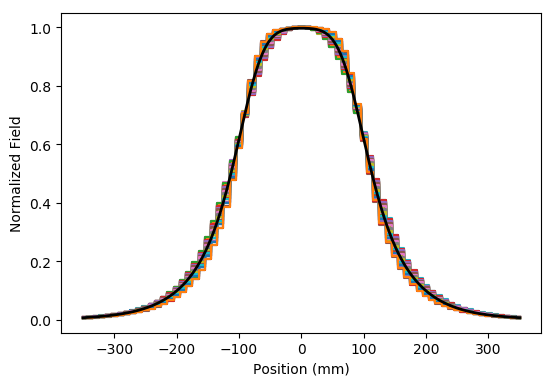
\includegraphics[width=0.85\textwidth]{figures/enge_fit.png}}
        \caption[Normalized field with Enge fit]{Normalized field and the
            resultant fit to the fringe field for the example quadrupole
            $Q_{10}$. The parameters of the fit are given in
            Table~\ref{tab:enge}.}
        \label{fig:enge_fit}
    \end{center}
\end{figure}

Using the field maps provided by Bruker, we can determine the Enge coefficients
and the effective field lengths for our magnets. For all calculations, since
the field near the center of the magnet is relatively weak, the fields within
2~cm in the radial direction of the central axis were not used for determining
either the effective field length or the Enge coefficients. Additionally, the
effective field length and the shape of the fringe field were assumed to not
differ with different magnet excitations, so all available data were used for
each magnet at the same time. An example using $Q_10$ of the normalized fields
used and the resulting fit is shown in Fig.~\ref{fig:enge_fit}.

The effective field lengths
were calculated directly from the field maps by integrating along the
$z$-direction for each radial distance provided. Since the maximum field
strength for a given magnet current varies depending on the distance from the
center, the individual ``traces'' of the magnetic field along the $z$-axis were
normalized. This normalization is shown in Eq.~\ref{eq:efl} as the constant
factor outside of the integral. The integration was performed using the
Simpson's Rule routine provided by the SciPy Python package~\cite{SciPy}. An
average of these lengths was used. Differences between the calculated effective
field length and those used within the initial ion optics solution were within
2\,\%. The new effective field lengths were used for all subsequent
calculations.

Using the same normalized field ``traces'' along the $z$-axis, the Enge
coefficients describing the shape of the fringe field may be determined. The
field profiles at each radial distance were fit simultaneously. Using the
default Enge coefficients as the initial parameter guesses, the summed mean
squared error between the data and Eq.~\ref{eq:shortquad} was minimized using
the Nelder-Mead downhill simplex minimization (see \cite{Simplex}) provided by
SciPy. The additional factor $k_0$ was included in the fit, but is not needed
when defining a fringe field within COSY. The process was repeated for each
quadrupole separately. The updated Enge coefficients and their comparison to
the default values used by COSY for $Q_{10}$ can be seen in Table~\ref{tab:enge},
and the difference in the shape of the fringe field can be seen in
Fig.~\ref{fig:enge_comparison}.

\begin{table}[t]
    \begin{center}
        \caption{ENGE COEFFICIENTS FOR $Q_{10}$ COMPARED TO COSY DEFAULTS}
        \label{tab:enge}
        \begin{tabular}{c S[table-format=2.8]S[table-format=2.6]}
            \toprule
            \midrule
            \textbf{Coefficient} & \textbf{$Q_{10}$ Values} &
                \textbf{COSY Defaults} \\
            \midrule
            $k_0$ &  0.99731489 & \\
            $a_0$ &  0.37255261 &  0.296471 \\
            $a_1$ &  6.18699778 &  4.533219 \\
            $a_2$ & -5.55514115 & -2.270982 \\
            $a_3$ &  6.96210851 &  1.068627 \\
            $a_4$ & -4.82581328 & -0.036391 \\
            $a_5$ &  1.3135787 &  0.022261 \\
            \bottomrule
        \end{tabular}
    \end{center}
\end{table}

\begin{figure}[t]
    \begin{center}
        \centerline{
            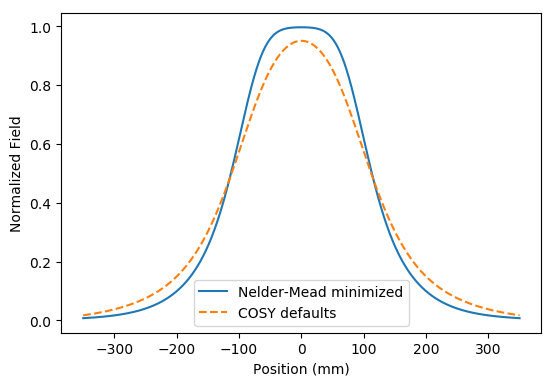
\includegraphics[width=0.85\textwidth]{figures/enge_comparison.png}}
        \caption[Comparison between fringe fields]{Comparison between fringe
            fields for the example quadrupole $Q_{10}$. The COSY default
            parameterization for the fringe field is the dashed orange line,
            and the fitted fringe field is the solid blue line. The distinct
            difference between the two field characterization requires the
            higher order effects arising from the fringe field to be taken into
            account.}
        \label{fig:enge_comparison}
    \end{center}
\end{figure}

In some cases, the field maps were not recorded far enough away from the center
of the magnet for the fitting routine to converge, primarily due to the field
not adequately reaching zero. In those cases, ``dummy'' points of zero field
were pre\---{} and post\---{}pended to the individual ``traces'' at distances
greater than 5~m from the center of the magnet to aide in convergence.

The default COSY coefficients for the fringe field were compared against the
data and shown to not adequately describe the field maps. The summed mean
squared error when using the short quadrupole formalization and the default
COSY parameters was significantly larger than that found through the
minimization routine, and the difference was shown to be statistically
significant. A visual comparison between the two models for $Q_{10}$ is shown
in Fig.~\ref{fig:enge_comparison}.


\section{Energy and Angular Acceptance}
\label{sec:commissioning}

The energy and angular acceptances of St.\ George were determined
experimentally through a series of experimental campaigns using multiple
rigidities. The energy acceptance without a corresponding angular acceptance
was shown to exceed the designed acceptance at zero degrees, with a measured
energy acceptance of $\Delta E/E = \pm 8$\,\% for ten different beam
rigidities covering the phase space region for astrophysically important
recoils~\cite{Meisel2017}. The angular acceptance has been shown to meet the
desired $\Delta\theta = \pm 40$~mrad in limited cases with an energy spread of
$\Delta E/E = \pm 3$\,\%. The full total acceptance has not yet been measured
within the designed phase space limits of St.\ George, with work ongoing.

Within the following discussion, the term ``test beam'' will be used in
reference to an incident beam produced by the 5U with a desired rigidity. These
test beams are defined by the beam particle, energy, and charge state selected
by the operator and produced by the 5U. These beams were chosen for to
provide particles with the desired rigidity and with beam currents in the range
of $0.5 - 3$~$\mu$A in order for the diagnostic equipment to properly measure
the beam. Additionally, those beams that commonly had highly stable 5U and ion
source running conditions over extended times were selected to reduce beam
preparation steps by the operators.

Acceptance measurements first probed the energy acceptance within the designed
$B\rho-E\rho$ phase space. The rigidity phase space
limits, along with measured acceptances and ranges for proposed future
experiments is shown in Figure~\ref{fig:rigidity-phase-space}. While it is not
possible to produce test beams with the 5U that completely span this phase
space, the regions of astrophysical interest are accessible, and work focused
on this region.

\begin{figure}[t]
   \begin{center}
       \label{fig:rigidity-phase-space}
       \centerline{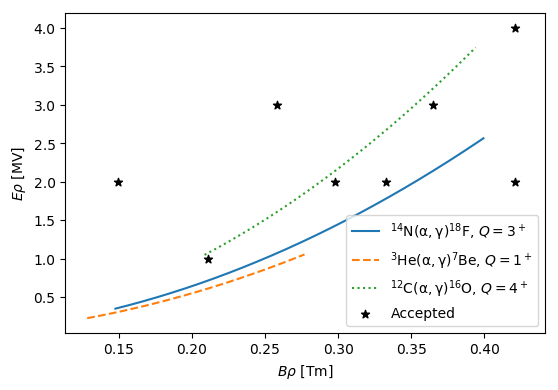
\includegraphics[width=0.8\textwidth]
           {figures/rigidity_phase_space.png}}
       \caption[Designed $B\rho-E\rho$ rigidity phase space for St.\ George]{
           Designed $B\rho-E\rho$ rigidity phase space for St.\ George. Stars
           represent rigidities that have been shown to have the full
           $\Delta E/E = 8$\,\% energy acceptance. Reactions shown are probable
           first experiments using St.\ George that use beam energies
           accessible with the 5U:
           \nuc{14}{N} at $E_{\rm{beam}}\approx 0.7-5.0$~MeV (solid blue line),
           \nuc{3}{He} at $E_{\rm{beam}}\approx 0.25-1.2$~MeV (dashed orange
           line), and
           \nuc{12}{C} at $E_{\rm{beam}}\approx 3.0-10.0$~MeV (dotted green
           line). These energy
           ranges cover some of the astrophysically important ranges for the
           given reactions.
           Adapted from~\cite{Meisel2017}.}
   \end{center}
\end{figure}


\subsection{Beam Tuning and Properties}
\label{sec:tuning}

The commissioning runs followed a similar procedure for beam preparation using
the 5U and the transport line. The beam rigidities were chosen to cover a
region within the phase space limits of the separator that cover recoils
produced through reactions of astrophysical interest. Both light (\nuc{1}{H}
and \nuc{4}{He}) and heavier (\nuc{16}{O} and \nuc{20}{Ne}) beams were used to
probe different regions of that phase space. Angular acceptance runs to date
have only used lighter beams. The energy uncertainty of the beam is
approximately 0.3~keV (see Section~\ref{sec:5U}), and a conservative value of
0.5~keV will be used when necessary.

Beam preparation can be divided into two segments: preparing the $\Delta E = 0$
test beam to enter into St.\ George along the central
magnetic optical axis, and transporting that beam along the central magnetic
optical axis within St.\ George. The following procedures were used for all
acceptance measurements, with differences being minor. The diagnostic equipment
described in Section~\ref{sec:diagnostic} was essential to performing the beam
preparation steps and their use is highlighted below.

\subsubsection{Before St.\ George}

The test beam must meet simple requirements in order to be useful for
commissioning St.\ George: it must enter St.\ George along the optical magnetic
axis, and it must have a narrow waist point with a circular cross section at
the target location. Additional requirements
were shown to be beneficial experimentally: the focus must not be highly
divergent, and the accelerator
must be providing highly stable beam current with low energy uncertainty. The
divergence of the beam was roughly known based on the focusing strength of the
preceding quadrupole magnets required to provide the desired beam properties
at the target location, with higher focusing strengths resulting in a more
divergent beam. A rough sketch of this relation is shown in
Figure~\ref{fig:divergence}.

\begin{figure}[t]
   \begin{center}
       \centerline{\includegraphics[width=0.8\textwidth]
           {figures/rigidity-phase-space.png}}
       \caption[Sketch of beam divergence due to focusing strength]{}
       \label{fig:divergence}
   \end{center}
\end{figure}

The beam intensity is dependent on which diagnostic equipment will primarily be
used. The isolated Faraday cups cannot read current below 50~$e$nA when read
through the logarithmic amplifier at the console,
and the current can't be above 20-30~$e\mu$A
as the cups are not currently water cooled and a high intensity and focused
beam may melt
some of the components. This upper current limit was not approached during the
tests, since the cups were used in tandem with the quartz viewers.
The quartz viewers are limited to
beam currents of a maximum of 3-5~$e\mu$A, as higher currents risk heating up
the quartz to
a high enough temperature to cause them to shatter or melt. Since four of the
quartzes
are also barriers between the high ($10^{-8}$~torr) vacuum within St.\ George
and atmosphere, this limit must be carefully avoided. In practice, currents
between 500~nA and 4~$\mu$A were used, based on the exact properties of the ion
source for that particular run, the beam species, and the locations of slits on
the primary transport line used to reduce the beam current.

The procedure for aligning the test beam to the magnetic optical axis is
described below. Major subsections of the procedure will begin with a short
title in bold to guide the reader. The elements on the main transport line that
may be necessary
to adjust are the switching magnet with the $X_6$ steerer, and the $Y_5$ and
$Y_6$ steerers (locations shown in Figure~[FIGURE]). The steerers are labeled
as such based on their position along
the main transport line. Steerers $X_6$ and $Y_6$ are part of the same physical
steerer but can be operated independently. Additionally, the quadrupole triplet
directly before the target location will be necessary for final tuning.

\textbf{Aligning the beam to St.\ George's optical axis:}
The desired test beam is transported down the St.\ George transport line and
monitored with the Faraday cup at the target location, called the
\emph{target cup} for beam current stability. Diagnostic equipment before the
target location are used as an aide to transport the beam and ensure that it
has the desired properties. If necessary, the beam current is reduced. The
quadrupole triplet is not be used at this point, since the beam may not be
entering the element along its magnetic optical axis.

The beam is sent into St.\ George. With no field in $Q_1$, $Q_2$, and $B_1$,
the beam hits the quartz viewer at the 0\degree{} exit port of the magnetic
vacuum chamber, called the \emph{$B_1$ quartz}. If the beam does not strike the
quartz, then the final set of steering elements needs to be adjusted to send
the beam into the quartz. When using the angular deflection commissioning
chamber, the current readbacks from the plates provides an additional
diagnostic on the trajectory of the beam.

\textbf{Checking for steering:}
Quadrupoles $Q_1$ and $Q_2$ are adjusted independently of each other, and the
resulting motion of the beam on the quartz is recorded. If the beam is aligned
with the central magnetic optical axis of either quartz, the quadrupole will
only focus the beam and not shift its position on the quartz, i.e.\ the spread
in the beam will
change but not its central position. The two quadrupoles must be adjusted
independently of each other as any induced steering from a beam misalignment in
one may be counteracted by a misalignment in the other quadrupole. If the beam
is steered by either quadrupole, the steering elements corresponding the the
focus direction of the offending quadrupole ($Y_5$ and $Y_6$ for $Q_1$, the
switching magnet and $X_6$ for $Q_2$) are adjusted to reduce the amount of
steering by that quadrupole.

A quadrupole steers a beam when the beam enters the magnetic element misaligned
with the optical magnetic axis. Assuming that the element is brought from zero
to defined strength, the focal length of the quadropule changes from
$\infty$ to a length $f$. The effect on the beam is that those regions of the
beam away from the optical axis are brought to pass through this focal point.
When a beam is aligned with the optical axis, there is an equal amount of the
beam on either side of this optical axis, so the beam spot will narrow along
the focusing axis of the quadrupole. The beam will also extend along the other
axis. If the beam is not aligned with the
optical axis, this beam motion to the focal point will be viewed as a lateral
motion along the focusing axis of the quadrupole.
A sketch of this effect can be seen in Figure~\ref{fig:steering}.

\begin{figure}[t]
   \begin{center}
       \centerline{\includegraphics[width=0.8\textwidth]
           {figures/rigidity-phase-space.png}}
       \caption[Sketch of quadrupole steering of misaligned beam]{}
       \label{fig:steering}
   \end{center}
\end{figure}

The goal for adjusting the steering elements before St.\ George is to have each
quadrupole induce no steering on the beam. In practice, each change to the
steering elements either increases or decreases the amount of steering in the
direction of that element.
The crossover point, where the beam switches from steering left to steering
right for example, can be used to restrict the possible phase space of steerer
values, as the beam must have a zero deflection position between those two
extremes.

While each direction should be independent of each other, if the beam is far
from the magnetic optical axis, a single quad may induce steering in both
directions. When minimizing steering in a single direction, say the
$x$-direction, the other direction must also be checked frequently.

At the end of this process, the beam is not deflected when the field strength
for either $Q_1$ or $Q_2$ is increased or decreased independently of the other
quadrupole. The beam may be said to be entering St.\ George along the optical
magnetic axis. Due to the short distance between the first quadrupole doublet
and the $B_1$ quartz, it may be necessary to increase the sensitivity of the
steering to ensure that we are as aligned as possible to the axis.

\textbf{Increase sensitivity:}
The beam is then sent further into St.\ George, first to the $B_2$ quartz
located within the beamline then the $B_3$ quartz. The steering of $Q_1Q_2$ is
again checked in the same fashion as before. As these quartzes are located
further from the quadrupoles, they give a higher sensitivity to steering
affects from misalignment than just using the $B_1$ quartz at the trade-off
that the the quadrupoles can only be set to lower field strengths. Since the
quartz is further from the focusing elements, the same focusing strength will
create a larger beam spot on the quartz viewer. This effect can be seen in
Figure~\ref{fig:steering}.

These additional checks require $B_1B_2$ to have field. While these two dipoles
must have an exact field strength when performing acceptance measurements or an
experiment, at this point their fields only need to be coarsely set such that
the beam strikes the desired quartz. While the higher order corrections from
these magnets do play a role in the direction and focusing of the beam, that
contribution has no effect on determining beam alignment within the
quadrupoles.

The steering elements are adjusted in the same fashion to minimize steering in
$Q_1Q_2$. Since this steering was minimized during the previous step, these
adjustments should be minimal. It may
be necessary to have a weak field in $B_3$ in order to see the beam on the
$B_3$ quartz, due to possible machining misalignments of the port that the
quartz is attached to and the residual magnetic field within the dipole.

\textbf{Include the quadrupole triplet:}
As the last focusing element before St.\ George, the quadrupole triplet
(henceforth simply the \emph{triplet}) is the final adjustable element to
determine the beam properties when entering the separator. The triplet is used
to focus the beam to a small spot at the target location, a requirement for
both experiments and acceptance measurements. As it and $Q_1Q_2$ should lie on
the same magnetic optical axis, its steering must also be checked and minimized
if its use is desired for the present experiment. It was not used in all cases
as the coarse target focus provided by the previous quadrupole doublets on the
main transport line were deemed sufficient.

Before moving the beam off of the $B_1$ quartz, the steering effects of the
triplet must be characterized in the same fashion as $Q_1Q_2$. During the
steering minimization steps, both the triplet and $Q_1Q_2$ must both be
minimally steering before moving forward.

Due to minor misalignments between the triplet and $Q_1Q_2$, it is usually not
possible to have all elements nonsteering at the same time. In these cases, the
steering of $Q_1Q_2$ should take precedence while having the triplet minimally
steering. While the steering of the beam prior to the target location is
important, experimentally the steering of the individual elements within the
triplet cancel or nearly cancel each other out when the triplet is minimally
steering, reducing that problem.

At this point, the main transport line has been tuned to prepare a well-focused
and well-aligned beam entering into St.\ George. These elements are not to be
touched during the rest of the tuning process. The triplet, due to the
possibility of it having minor steering effects, must also have zero field for
the remainder of the steering checks, and will be turned on for the actual
measurement.

\subsubsection{Within St.\ George}
\label{sec:tuning_stg}

Once the test beam has been aligned to enter the separator along the magnetic
optical axis, it must also be aligned to the magnetic optical axes of all of
the quadrupoles within the separator. This alignment is done using only the
dipoles $B_{1-6}$ and the WF. Any minor misalignment in the vertical
direction should have been corrected during the previous steps, but there is
the possibility that there will be vertical steering within the separator, both
from that misalignment and effects from the dipoles and
quadrupoles. Within St.\ George, this equates to the $y$-focusing quadrupoles
($Q_{1,\,4,\,7,\,8,\,11}$) potentially steering minorly in the vertical
direction despite the best efforts of the operator. As there are no elements
within St.\ George that could correct for this, the steering effect of these
quadrupoles may not be able to be eliminated. The procedure for this second
alignment is straightforward, as the
only elements used to adjust the steering of the quadrupoles are the two
dipoles immediately prior.

\textbf{Tuning to the WF:}
With the beam striking the $B_3$ quartz, quadrupoles $Q_{3-5}$ are checked for
steering. The primary focus of these steering
checks will be on $Q_3$ and $Q_5$ which focus in the horizontal plane. The
magnetic fields within $B_1B_2$ are
adjusted to make these quadrupoles non-steering or minimally steering. The
field precision is on the order of 0.1~G, read back by the Hall probes.

Due to potentially small misalignments in the St.\ George quadrupoles in
relation to each other, it is commonly not possible to have $Q_{1-5}$
non-steering simultaneously (see \cite{Meisel2017}). In these cases, minimal
steering can be achieved through $Q_{3-5}$ when $Q_1Q_2$ are non-steering by
adjusting $B_1B_2$. At this point, dipoles $B_1B_2$ are set to the value
corresponding to the magnetic rigidity of the particle and to maintain the
test beam alignment to the optical axis.

Dipoles $B_3B_4$ are brought up to their rough field value to send the beam
through the WF and onto either the WF quartz or the $B_5$ quartz. The
quadrupoles $Q_{6-9}$ are checked for steering, adjusting $B_3B_4$ to minimize
the steering. Since there is some residual magnetic field within the Wien
filter, the electric field is brought up to compensate for this bending to keep
the test beam along the optical axis through $Q_8Q_9$. The field required is
calculated by determining the bending radius caused by the residual magnetic
field and creating the equivalent bending radius in the opposite direction for
the particle's $E\rho$.

As the beam envelope has expanded, it will be necessary to bring $Q_{1-5}$ to
their desired values in order to check the steering of the remaining
quadrupoles. Since these quadrupoles have been shown to be minimally steering,
their effect on the beam trajectory through remainder of St.\ George should be
negligible. It may be necessary to have a weak field in $B_5$ in order to see
the beam on the $B_5$ quartz for the same reasons as explained previously for
$B_3$.

\textbf{Setting the WF:}
For a test beam with $\Delta E = 0$ and $\Delta\theta = 0$, the elements within
St.\ George will be set to transport this along the central axis based on the
test beam's rigidity. Since the energy of the beam is well known and the charge
of the beam is exact, the electric rigidity $E\rho$ is also well known. The
electric dipole within the WF is set for this rigidity and held
constant for the remainder of the tuning process.

The magnetic field is set similarly to the other dipoles: to minimize the
steering induced by the next set of quadrupoles ($Q_8Q_9$). Since the test beam
was aligned to the optical magnetic axes of this quadrupole doublet in the
previous step, the WF magnetic dipole must return the beam to this
orientation. Additionally, since the elements within St.\ George act to
prepare the beam to be separated by mass by the WF, the quadrupoles
$Q_{1-7}$ must be set to the values determined by the test beam's magnetic
rigidity $B\rho$.

The magnetic field for the WF is read back using a Hall probe located
on the pole face. The field can be set precisely and related to the fields in
the other dipoles. Once the magnetic field is set such that $Q_8Q_9$ do not
steer the beam, the full WF is set.

\textbf{Tuning through the detector chamber:}
Dipoles $B_5B_6$ are set to their rough values based on the $B\rho$ of the test
beam, sending the beam through the detector chamber and onto the last quartz,
called the \emph{detector quartz}. As before, due to the size and shape of the
beam envelope, $Q_8Q_9$ must be set to the required values. The final two
quadrupoles $Q_{10}Q_{11}$ are checked for steering, and $B_5B_6$ are adjusted
to minimize that steering.

Since the test beam is traveling through the detector chamber, the entire
detection system must be pulled out of the way of the beam. Magnetic shields
have been placed below the MCP constructs to remove the effect of the magnetic
fringe fields on the beam deflection~\cite{MoralesDNP}. Once $Q_{10}Q_{11}$ are
non-steering, the test beam is fully aligned to the optical magnetic axis of
St.\ George.

\subsubsection{Collimator and Target Position}

The 2~mm diameter collimator at the target location
(see Section~\ref{sec:target}) is
used for setting the triplet to the proper values. A narrow waist beam at the
target location is a requirement to achieve the maximum angular and energy
acceptance
for St.\ George. With the collimator in place, the triplet is adjusted such
that the beam transmission, defined as the ratio between the beam currents
before and after the collimator as read by two separate Faraday cups, is
maximized and ideally close to 100\,\%.

Since the target chamber may rotate around its central axis, it is possible for
the location of the collimator to become slightly misaligned between runs.
Additionally,
the triplet may induce some minor steering at the target location, potentially
moving the focal point radially from the optical magnetic axis. The target
collimator position is then not a fixed value but must also be tuned to
maximize transmission. Once the collimator position is found, the target
position is immediately known.

Rotation angles between $-5$ and $+25$\degree{}, where 0\degree{} is to the
right from the beam's perspective, and extensions of $91-96$~mm of the mounted
linear motion have been explored. Maximum transmission has been found for
collimator positions within this range of rotation angles and extension
distances for multiple beams, restricting
the total possible search space for the collimator. Extensions of the
target ladder of $\approx 94$~mm, and rotation angles near $+10$\degree{} are
common ``best positions'' for the collimator.

For acceptance measurements, the collimator is used to create a focal point at
the target location. Once the beam preparation is complete, it is retracted
from the beamline. When a target is used as a degrader, the collimator position
is used to determine the target position.


\subsection{Energy Acceptance}

The energy acceptance of St.\ George at $\Delta\theta = 0$~mrad was measured to
be $\Delta E/e = \pm 8$\,\% for ten different rigidities (see
Fig.~\ref{fig:rigidity-phase-space} and \cite{Meisel2017}). The measurements
took place before the capability to measure the angular acceptance and will
be remeasured as part of a total acceptance measurement campaign. Test beam
rigidities were chosen to cover an adequate region within the designed phase
space near the rigidities expected for recoils of astrophysical interest and
based on the restrictions imposed by the 5U and ion source.

For a given set of field settings for a test beam at $\Delta E = 0$ that
provide 100\,\% transmission between the target cup and a Faraday cup located
within the detector chamber at focal plane $F_3$, the separator is said to
accept an energy difference if the test beam is changed to that different
energy and still have 100\,\% transmission between those two cups. To state that
St.\ George has an energy acceptance of $\Delta E/E = \pm 8$\,\%, a single set of
fields for the elements within the separator transmitted 100\,\% of the test beam
between the two cups when its energy was changed within that energy change.

The procedure for measuring the energy acceptance of a single rigidity is
outlined below. The slits located at the post-WF focal plane $F_2$
were used to define a beam center. As the tune for a given recoil is supposed
to be achromatic at this location, these slits were used as both a diagnostic
on the path of the beam and a check of this requirement during the
measurements. Note that the tuning process for these measurements did not make
use of the in-beam quartz viewers at $F_1$ and $F_2$ since they had not yet
been installed.

\textbf{Initial setup:}
After tuning a beam along the optical magnetic axis as described in
\ref{sec:tuning}, all elements within St.\ George are at a given field. The
dipole elements, including the WF, are not touched. The transmission
between the target cup and the $F_3$ cup is measured. If the transmission is
100\,\%, the beam energy was changed. If not, then the quadrupoles were retuned
to transmit 100\,\% of the test beam between the two cups.

Quadrupole retuning was done systematically to prevent over- or under-focusing
the beam at any location within St.\ George. With the beam on the $F_3$ cup,
each quadrupole was adjusted individually to determine what field is required
to transmit 100\,\% of the beam to the cup. After finding that field, the
difference is recorded and the quadrupole is returned to its original value.
This process is repeated for every quadrupole acting independently. If a single
quadrupole could not achieve 100\,\% transmission on its own, it was not included
in the next step. Assuming $N$ quadrupoles adjusted by $\Delta B_i$ to give
100\,\% transmission, the individual quadrupoles $Q_i$ were changed by
$\Delta B_i / N$. This approach usually resulted in achieving 100\,\%
transmission for the $\Delta E = 0$ case.

The quadrupole adjustment described was used at every step if the tune was
shown to not transmit 100\,\% of the test beam. Previous settings of the
quadrupoles were recorded to map regions of field strengths were 100\,\%
transmission was achieved for different energy changes.

\textbf{Changing energy:}
The beam energy was changed to $\Delta E/E = -8$\,\% by changing the accelerator.
The transport beamline was scaled automatically to account for the change in
rigidity. The beam was shown to enter into St.\ George along the optical
magnetic axis by putting the fields within $Q_1$, $Q_2$, and $B_1$ to zero and
checking the steering of the first two quadrupoles. Since this energy change is
minor, in most cases only the switching magnet needed to be changed. The
magnets $Q_1Q_2B_1$ were brought back to their required values and transmission
between the two cups was checked.

If the beam was fully transmitted to the $F_3$ cup, the settings for St.\
George were said to have an energy acceptance of $\Delta E/E = -8$\,\%. The beam
energy was then changed to $\Delta E/E = + 8$\,\%, following the same procedure,
and transmission was checked. If the beam also was fully transmitted, the
separator tune was said to have an energy acceptance of $\Delta E/E = \pm 8$\,\%
and the measurement was complete.

Where 100\,\% transmission was not achieved, the quadrupole scaling described
previously was used. The new tune was recorded, and the beam energy was
returned to $\Delta E = 0$ to check transmission. This process was continued
until all three energy points had 100\,\% transmission for a single setting of
St.\ George. During this cycling, referring to previous values was used to
prevent correcting the tune in one direction at one energy only to change back
to the previous tune at another energy.

Since the $F_2$ slits were placed around the beam center, achieving 100\,\%
transmission was only possible if test beam had a nearly or completely
achromatic focus following the WF, one of the requirements for normal
operation of the separator.

\textbf{Additional measurements:}
For subsequent energy acceptance measurements, instead of using the COSY
predicted values, an energy acceptance tune scaled based on the magnetic
rigidity $B\rho$ of the new test beam was used for the initial quadrupole
settings. If the difference in $B\rho$ was sufficiently small, the required
adjustments to the quadrupole fields were minimal, speeding up the measurement
process. As more individual energy acceptance measurements were made, the
scaling based on $B\rho$ became more robust to slight differences in beam
preparation and species.

Once the ten rigidities within the astrophysically interesting phase space of
the separator were measured, work moved to measuring the angular acceptance.


\subsection{Angular Acceptance}

As of this writing, the angular acceptance of St.\ George has been measured to
be $\Delta\theta = \pm 40$~mrad in the horizontal and vertical planes for a
single rigidity. The acceptance was shown by ensuring 100\,\% transmission
when deflecting the beam 40~mrad in each direction, and quadrupole adjustments
followed the same procedure as during the energy acceptance measurements. The
measurement was done without a corresponding energy acceptance, and without the
requirement that the test beam be focused at the focal plane $F_2$ following
the WF and without the beam passing through the slit opening at that
location for all deflection angles. The measurement was then a single ``proof
of concept'' that an angular acceptance could be measured using the new
diagnostic and control equipment installed. Due to complications with the
measurement process, multiple attempts at measuring the angular acceptance,
each with a different procedure, were tried. These attempts are outlined below.

\textbf{Deflector plates only:}
A test beam is tuned to provide a non-steering beam with 100\,\% transmission
between the target and $F_3$ cups. The deflector plates (see
Section~\ref{sec:target}) are rotated so that they deflect the beam in a single
plane. The horizontal plane was commonly chosen first. Since the entrance
aperture for the target cup is larger than 40~mrad, it does not intercept any
of the beam when it is deflected. Angles between 0 and 40~mrad were used and
the current on the $F_3$ cup was monitored. The maximum angle that provided
100\,\% transmission was recorded.

If the maximum angle achieved was not 40~mrad, the quadrupoles were tuned in
the same fashion as for the energy acceptance measurement but with the
deflector plate set to an angle greater than was accepted such that the beam
is still partially captured by the cup. The changes to the quadrupole fields
were recorded, and all quadrupoles that could provide 100\,\% transmission were
scaled to new values. The beam was returned to $\Delta\theta = 0$ to ensure
that the new tune still provided 100\,\% transmission in this case, and the
deflection was changed.

A single plane was checked for $\pm 40$~mrad first before switching to the
other plane, and any retuning was done to also transmit 100\,\% of the beam to
the final cup. The deflector was also rotated to check the other plane, and
the quadrupoles retuned to provide 100\,\%. In general, this procedure did not
provide 100\,\% transmission when deflecting a test beam up to 40~mrad in the
four cardinal directions. This procedure was used for the single full angular
acceptance measurement.

Additionally, since the angular and energy acceptance is dependent on the
beam extent and shape at focal plane $F_2$, the WF quartz was used to
aide in tuning $Q_{1-7}$ to their proper values. The beam should move minimally
at this location when deflected up the the maximum 40~mrad in any direction.
The beam profile is required to be horizontally narrow for the highest mass
separation, requiring the vertical extent to be large. Using this intermediate
quartz slightly improved the ability to tune the separator but did not allow
for a full angular acceptance measurement to be performed.

\textbf{Degrader foil:}
The limiting factor in using the deflector plates as the only angular change is
that each direction must be looked at independently. Assuming the plates are
aligned to deflect in the horizontal direction, only one direction (left or
right from the beam's perspective) can be viewed at a time without some
manual adjustment to the deflector plate power supply. The cyclic problem of
correcting the beam trajectory only to remove that correction becomes harder to
avoid. Since the plates can only deflect along a single plane, the additional
unknowns of removing a large angular acceptance along a difference by making
changes on the current plane also decreased the possibility of success.

At the target location, Al foils of different thicknesses were placed to
degrade the beam, creating a spread in angle and energy at the same time. Foil
thicknesses were matched with beam properties to fall within the anticipated
$\Delta E/E = \pm 8$\,\% and $\Delta\theta = \pm 40$~mrad acceptances of St.\
George. Since the foils also induce an energy loss for the test beam, the
separator dipoles needed to be properly scaled down to the correct values after
the test beam (without foil in place) was aligned to the magnetic optical axis.
The scaling required accurate and precise measurements of the foil thicknesses.
Thicknesses ranged from $100-250$~$\mu$g/cm$^2$, and \nuc{1}{H} and \nuc{4}{He}
test beams in the energy range of $0.9-2.0$~MeV were used.

Using the WF quartz, the test beam was tuned to have the correct phase space
properties at $F_2$. The degraded test beam is emitted into the separator
within a phase space determined by its interaction with the foil, allowing the
magnets to be tuned without relying on the slow change between deflection
angles and directions and including the minor energy acceptance measurement.
Currently, no full angular acceptance measurements have been made past $F_2$.

% Dalmore 12 Year - The Exchange

\textbf{Reaction Measurement:}
Additional measurements have been made of the angular acceptance with an
energy acceptance and a nearly achromatic focus at the $F_2$ focal plane. These
measurements were for the altered settings for transporting $\alpha$ particles
from $(\textrm{p},\alpha)$ reactions. The measurements are a different ``proof
of concept'' for the angular acceptance measurements by verifying a
$\Delta\theta = \pm 40$~mrad acceptance with the deflector plates before using
a foil to produce the full angular spread. In this case (see [SECTION]), the
transported particles are the reaction product $\alpha$ particles, verified
using a direct test beam of $\mnuc{4}{He}^{2+}$. The transported reactions
products within the $\approx 45$~mrad cone limited by the target Faraday cup were
transported to $F_2$ and detected with the Si detector.


\section{Considerations}

Full acceptance measurements require a fine detailed understanding of the
operation of St.\ George. Previous work has provided the initial understanding
on providing a large energy acceptance of at least $\Delta E/E = \pm 8$\,\% and
angular acceptances near $\Delta\theta = \pm 40$~mrad. Combined measurements
have been limited to a large energy acceptance and small angular acceptance or
vice versa. Current work is ongoing on providing an improved understanding of
the operation of St.\ George, particularly in setting the quadrupole fields.

A full commissioning of the separator system requires the gas target,
separator, and detection system to be operated in parallel and well-understood.
The current status of each of these discrete systems is varied. The Hippo gas
target has been tested in a prior configuration, and work has been started to
redesign the upper chamber to improve the possibility for monitoring incident
beam current and using a $\gamma$ detector in coincidence with the final
detector system. The combined $E_{\rm{TOTAL}} vs. TOF$ detection system has
been shown to work for test surface sources. Silicon detectors are known to be
very robust, and the Si detector and acquisition system has been used for
a successful measurement with St.\ George for $(\rm{p},\alpha)$ measurements.
The separator status has been explored earlier in this chapter. Final
verification of the separator will be measuring the test reaction
\react{\mnuc{14}{N}}{\alpha}{\gamma}{\mnuc{18}{F}} in inverse kinematics.

The target chamber used for the commissioning work and the experimental
campaign is different than that which will be used during a fully featured St.\
George experimental campaign, namely the Hippo supersonic helium gas jet
target. Hippo will be used for $(\alpha,\gamma)$ experiments following the
completion of the commissioning work. The specifics of that gas target are
discussed elsewhere (see \cite{Kontos2012} and \cite{Meisel2016}). Due to the
differences between the commissioning chamber and the design of the gas target,
some specifics of beam tuning and preparation (see Sec.~\ref{sec:tuning}) will
inevitably change as experimental work transitions between commissioning and
reaction research work.
